\chapter{Membangun Model Prediksi}

Untuk pratikum saati ini menggunakan buku \textit{Python Artificial Intelligence Projects for Beginners}\cite{eckroth2018python}. Dengan praktek menggunakan python 3 dan editor anaconda dan library python scikit-learn.
Dataset ada di https://github.com/PacktPublishing/Python-Artificial-Intelligence-Projects-for-Beginners .
Tujuan pembelajaran pada pertemuan pertama antara lain:
\begin{enumerate}
\item
Mengerti implementasi klasifikasi
\item
Memahami data set, training dan testing data
\item
Memahami Decission tree.
\item
Memahami information gain dan entropi.
\end{enumerate}
Tugas dengan cara dikumpulkan dengan pull request ke github dengan menggunakan latex pada repo yang dibuat oleh asisten riset. Kode program menggunakan input listing ditaruh di folder src ekstensi .py dan dipanggil ke latex dengan input listings. Tulisan dan kode tidak boleh plagiat, menggunakan bahasa indonesia yang sesuai dengan gaya bahasa buku teks.

\section{Teori}
Praktek teori penunjang yang dikerjakan(nilai 5 per nomor, untuk hari pertama) :
\begin{enumerate}
\item
Jelaskan apa itu binary classification dilengkapi ilustrasi gambar sendiri
Binary classification
Klasifikasi biner mengacu pada tugas-tugas klasifikasi yang memiliki dua label kelas.
Contohnyameliputi:
Deteksi spam email (spam atau tidak).
Prediksi churn (churn atau tidak).
Prediksi konversi (beli atau tidak)
\begin{figure}[!htbp]
	\centering
	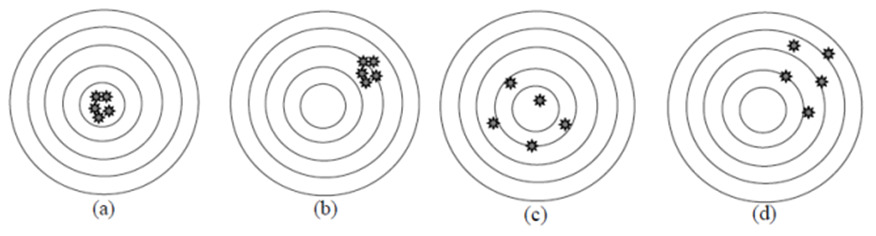
\includegraphics[scale=0.4]{figures/chapter 2/13.PNG}
\end{figure}

\item
Jelaskan apa itu supervised learning dan unsupervised learning dan clustering dengan ilustrasi gambar sendiri.
clustering 
adalah proses mengelompokkan data kedalam beberapa cluster atau kelompok sehingga data dalam suatu clsuter memiliki tingkat kemiripan yang maksimum dan data antar cluster yang berbeda memiliki kemiripan minimum.
supervised learning
pendekatan untuk menciptakan kecerdasan buatan ( AI ), di mana algoritmakomputerdilatih pada data input yang telah diberi label untuk output tertentu. Model dilatih hingga dapat mendeteksi pola dan hubungan yang mendasari antara data input dan label output, memungkinkannya menghasilkan hasil pelabelan yang akurat saat disajikan dengan data yang belum pernah dilihat sebelumnya.
un-supervised learning
menggunakan algoritme pembelajaran mesin untuk menganalisis dan mengelompokkan kumpulan data yang tidak berlabel. Algoritma ini menemukan polater sembunyi atau pengelompokan data tanpa perlu campu rtangan manusia.

\item
Jelaskan apa itu evaluasi dan akurasi dari buku dan disertai ilustrasi contoh dengan gambar sendiri
Evaluasi 
evaluasi ini merupakan suatu proses merencanakan, memperoleh, serta juga menyediakan informasi yang sangat diperlukan untuk dapat membuat alternatif-alternatif keputusan.

Akurasi 
\begin{figure}[!htbp]
	\centering
	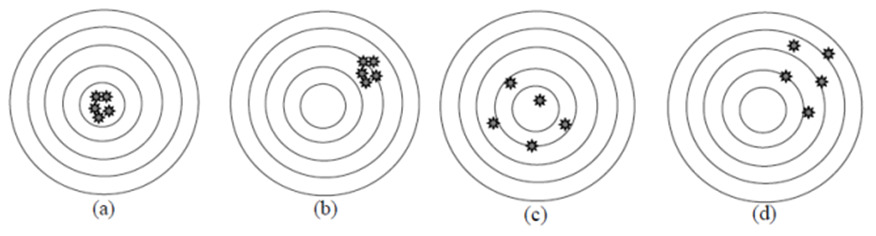
\includegraphics[scale=0.4]{figures/chapter 2/13.PNG}
\end{figure}
 

Pada Gambar di atas terdapat 4 buah kondisi ketika kita menembakkan beberapa perluru pada sebuah sasaran. Tujuan kita disini adalah untuk menembak bagian tengah sasaran tersebut.Pada Gambar (a) dan (c) pada Gambar di atas merupakan gambar yang menunjukkan seseorang telah berhasil mengenai bagian tengah sasaran tersebut dapat kita katakan pula tembakan pada kedua gambar tersebut akurat. Akurat dalam hal ini dapat diartikan suatu kondisi dimana kedekatan lubang peluru dengan pusat sasaran. Secara umum akurasi diartikan sebagai tingkat kedekatan pengukuran kuantitas terhadap nilai sebenarnya.

\item
Jelaskan bagaimana cara membuat dan membaca confusion matrix, buat confusion matrix buatan sendiri.
Confusion matrix 
 cara membuat dan membaca 
a.	Menentukan masalah dan atribut yg dibutuhkan, contohnya gaji atau listrik
b.	Buat pohon keputusan
c.	Buat data testingnya

\item
Jelaskan bagaimana K-fold cross validation bekerja dengan gambar ilustrasi contoh buatan sendiri.
K-Fold Cross Validation
suatu metode tambahan dari teknik data mining yang bertujuan untuk memperoleh hasil akurasi yang maksimal. Metode inisering juga disebut dengan k-fold cross validation dimana percobaan sebanyak k kali untuk satu model dengan parameter yang sama

\item
Jelaskan apa itu decision tree dengan gambar ilustrasi contoh buatan sendiri.
\item
Jelaskan apa itu information gain dan entropi dengan gambar ilustrasi buatan sendiri.
information gain  Data yang diperoleh saat penurunan data set dibagi berdasarkan atribut. 
Entropy mengukur ketidakpastian suatu variabel acak. Misal kita punya uang logam, jika kita lempar kita tidak memiliki kepastian apakah yang diperoleh gambar atau angka.



\end{enumerate}

\section{scikit-learn}
Dataset ambil di https://github.com/PacktPublishing/Python-Artificial-Intelligence-Projects-for-Beginners folder Chapter01.
Tugas anda adalah, dataset ganti menggunakan \textbf{student-mat.csv} dan mengganti semua nama variabel dari kode di bawah ini dengan nama-nama makanan (NPM mod 3=0), kota (NPM mod 3=1), buah (NPM mod 3=2), . Jalankan satu per satu kode tersebut di spyder dengan menggunakan textit{Run current cell}. Kemudian Jelaskan dengan menggunakan bahasa yang mudah dimengerti dan bebas plagiat dan wajib skrinsut dari komputer sendiri masing masing nomor di bawah ini(nilai 5 masing masing pada hari kedua).

\begin{enumerate}

\item
\begin{verbatim}
	# load dataset (student mat pakenya)
	import pandas as pd
	d = pd.read_csv('student-mat.csv', sep=';')
	len(d)
\end{verbatim}
\begin{figure}[!htbp]
	\centering
	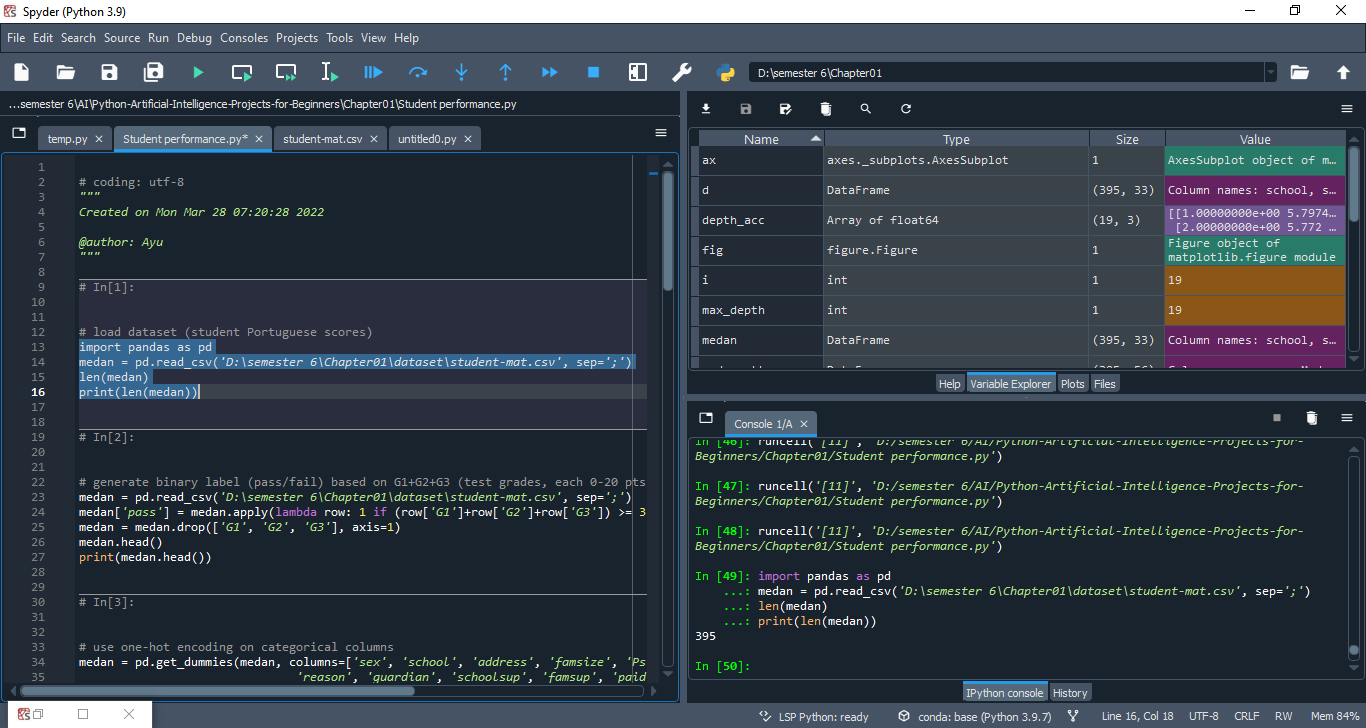
\includegraphics[scale=0.4]{figures/chapter 2/1.PNG}
\end{figure}
\newpage
\item
\begin{verbatim}
	# generate binary label (pass/fail) based on G1+G2+G3 
	# (test grades, each 0-20 pts); threshold for passing is sum>=30
	d['pass'] = d.apply(lambda row: 1 if (row['G1']+row['G2']+row['G3']) 
											>= 35 else 0, axis=1)
	d = d.drop(['G1', 'G2', 'G3'], axis=1)
	d.head()
\end{verbatim}
\begin{figure}[!htbp]
	\centering
	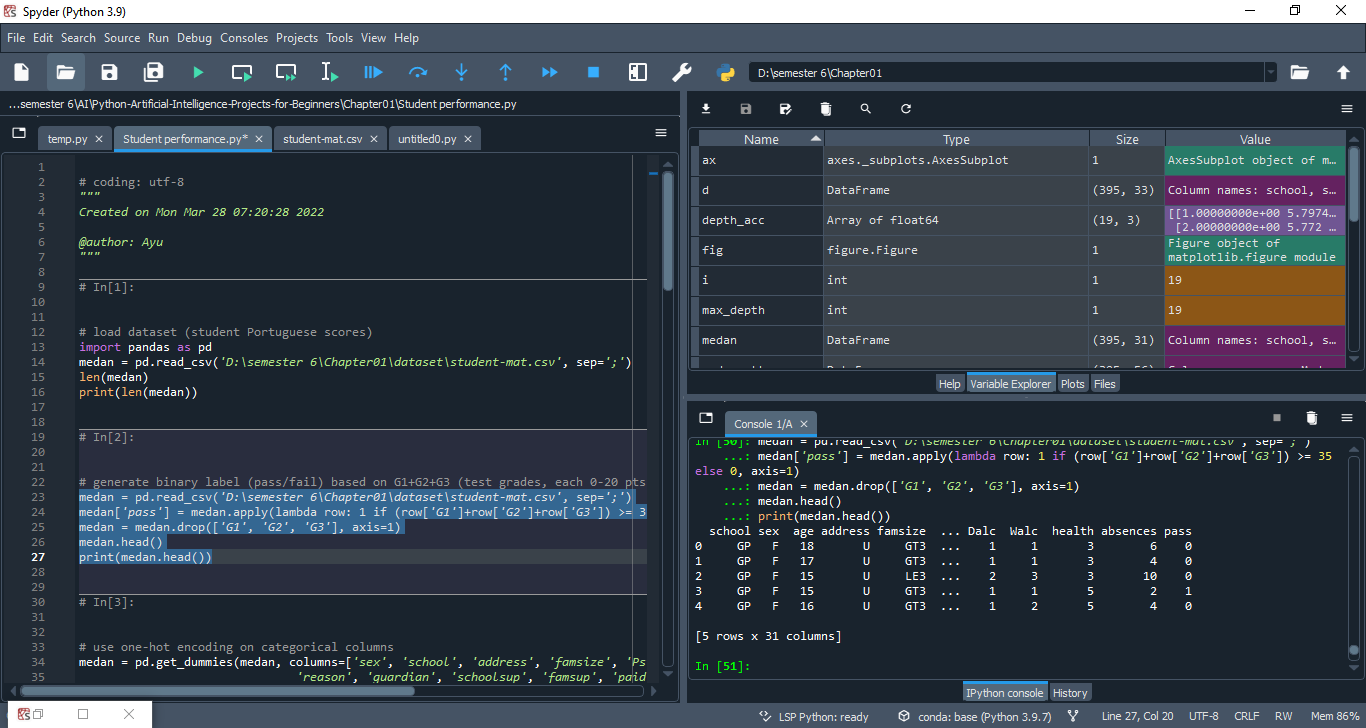
\includegraphics[scale=0.4]{figures/chapter 2/2.PNG}
\end{figure}
\newpage
\item
\begin{verbatim}
	# use one-hot encoding on categorical columns
	d = pd.get_dummies(d, columns=['sex', 'school', 'address', 
									'famsize', 
									'Pstatus', 'Mjob', 'Fjob', 
	                               'reason', 'guardian', 'schoolsup', 
								   'famsup', 'paid', 'activities',
	                               'nursery', 'higher', 'internet', 
									'romantic'])
	d.head()
\end{verbatim}
\begin{figure}[!htbp]
	\centering
	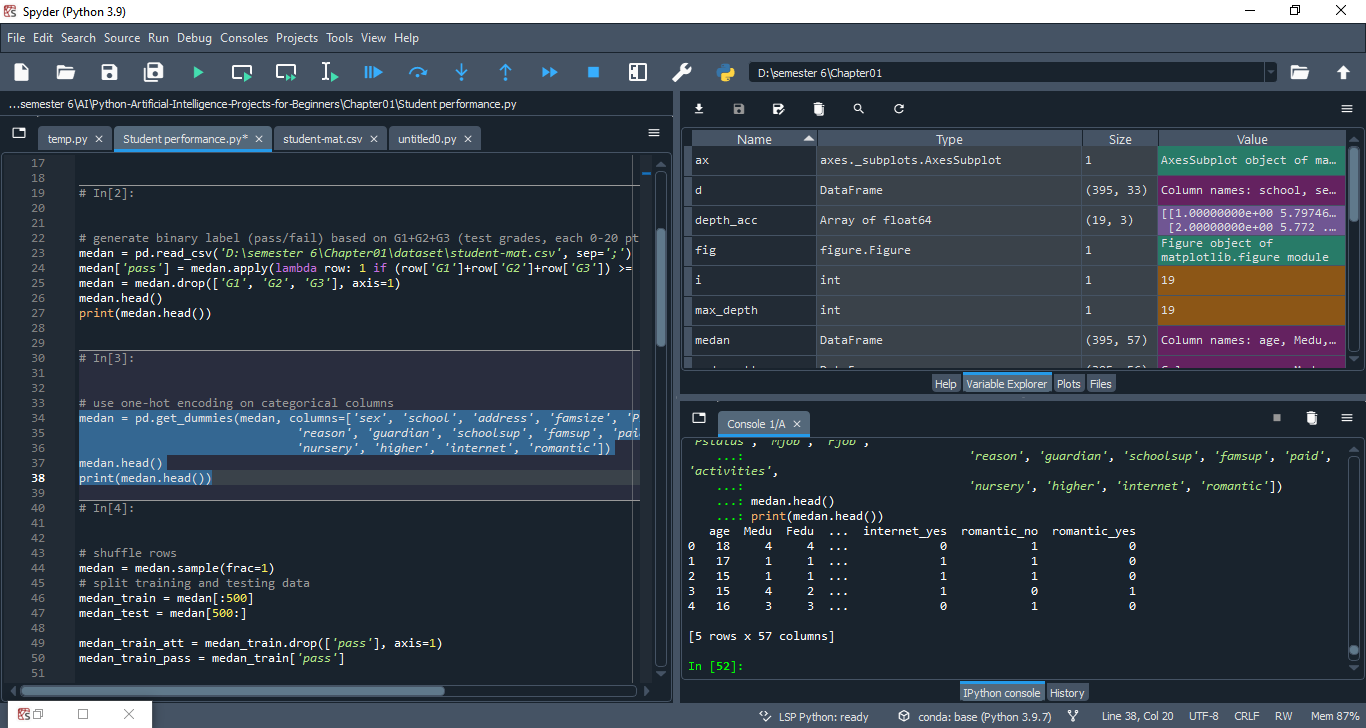
\includegraphics[scale=0.4]{figures/chapter 2/3.PNG}
\end{figure}
\newpage
\item
\begin{verbatim}
	# shuffle rows
	d = d.sample(frac=1)
	# split training and testing data
	d_train = d[:500]
	d_test = d[500:]

	d_train_att = d_train.drop(['pass'], axis=1)
	d_train_pass = d_train['pass']

	d_test_att = d_test.drop(['pass'], axis=1)
	d_test_pass = d_test['pass']

	d_att = d.drop(['pass'], axis=1)
	d_pass = d['pass']

	# number of passing students in whole dataset:
	import numpy as np
	print("Passing: %d out of %d (%.2f%%)" % (np.sum(d_pass), len(d_pass), 
	       100*float(np.sum(d_pass)) / len(d_pass)))
\end{verbatim}
\begin{figure}[!htbp]
	\centering
	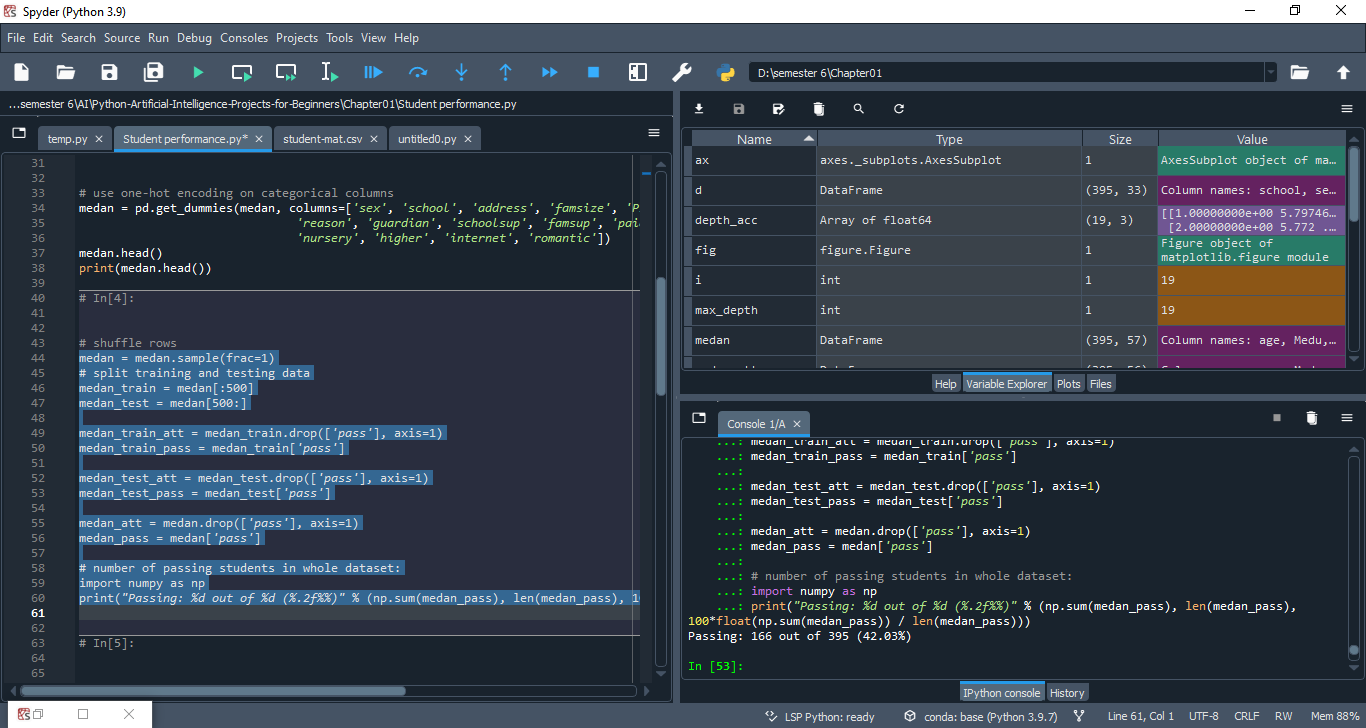
\includegraphics[scale=0.4]{figures/chapter 2/4.PNG}
\end{figure}
\newpage
\item 
\begin{verbatim}
	# fit a decision tree
	from sklearn import tree
	t = tree.DecisionTreeClassifier(criterion="entropy", max_depth=5)
	t = t.fit(d_train_att, d_train_pass)
\end{verbatim}
\begin{figure}[!htbp]
	\centering
	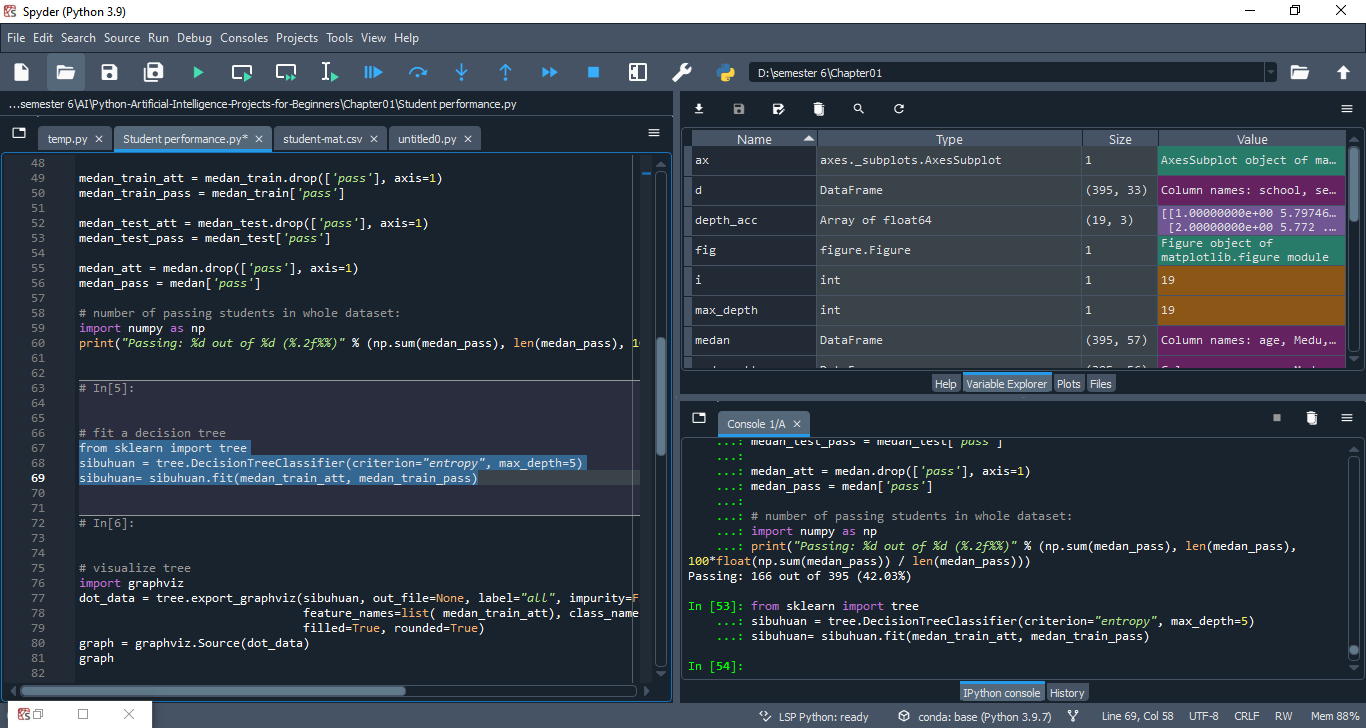
\includegraphics[scale=0.4]{figures/chapter 2/5.PNG}
\end{figure}
\newpage
\item
\begin{verbatim}
	# visualize tree
	import graphviz
	dot_data = tree.export_graphviz(t, out_file=None, label="all", 
									impurity=False, proportion=True,
	                                feature_names=list(d_train_att), 
									class_names=["fail", "pass"], 
	                                filled=True, rounded=True)
	graph = graphviz.Source(dot_data)
	graph
\end{verbatim}
\begin{figure}[!htbp]
	\centering
	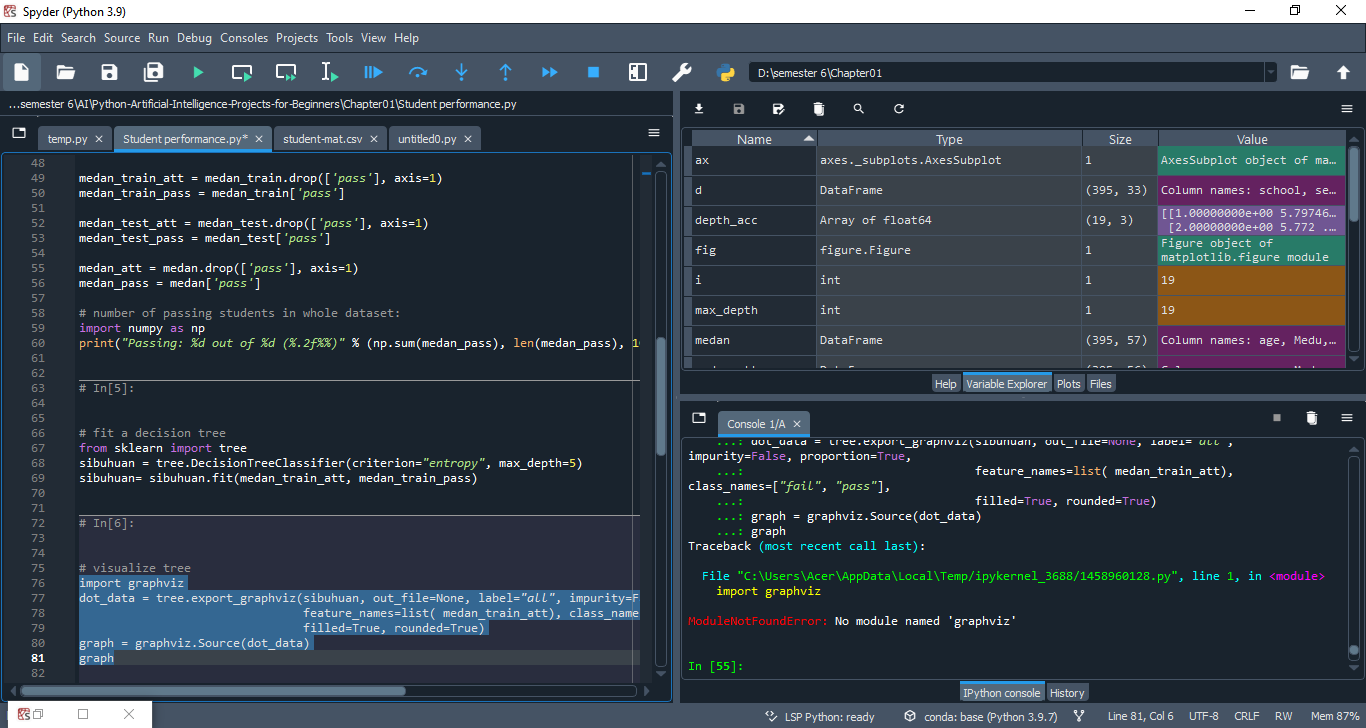
\includegraphics[scale=0.4]{figures/chapter 2/6.PNG}
\end{figure}
\newpage
\item
\begin{verbatim}
	# save tree
	tree.export_graphviz(t, out_file="student-performance.dot", 
						 label="all", impurity=False, 
						 proportion=True,
	                     feature_names=list(d_train_att), 
	                     class_names=["fail", "pass"], 
	                     filled=True, rounded=True)
\end{verbatim}
\begin{figure}[!htbp]
	\centering
	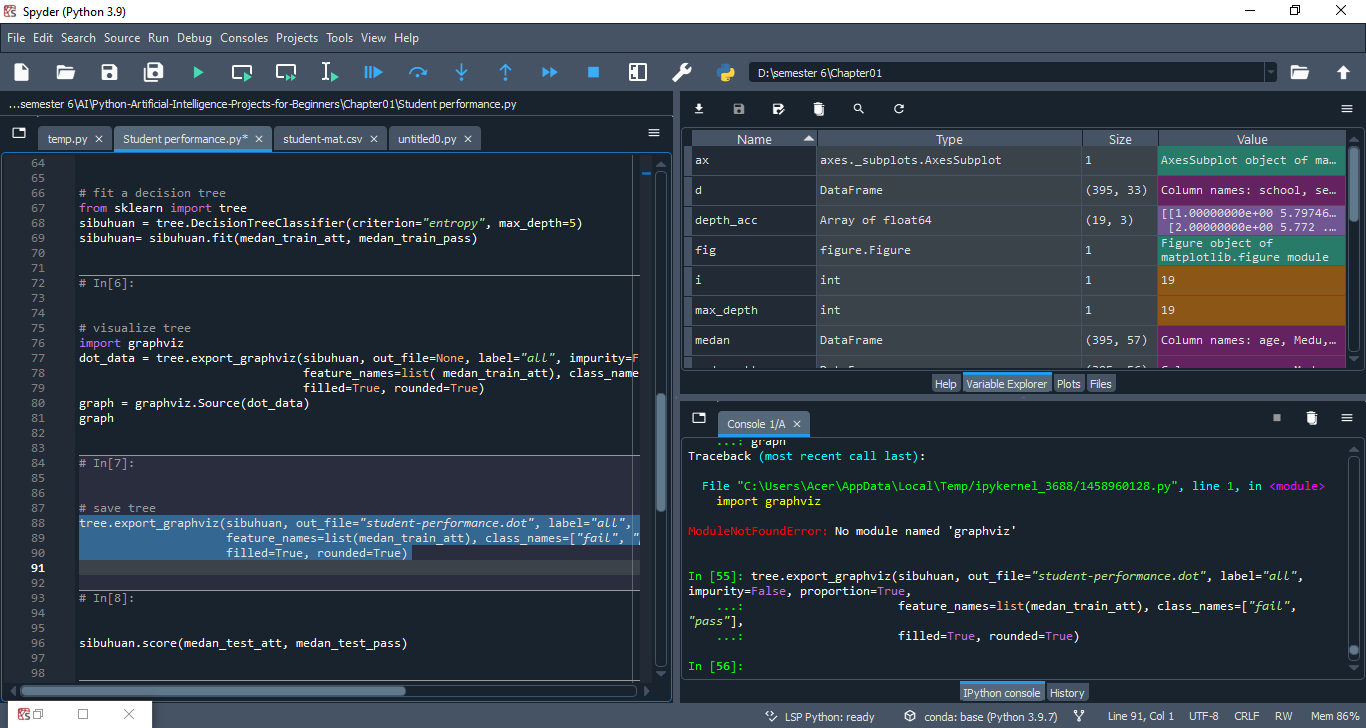
\includegraphics[scale=0.4]{figures/chapter 2/7.PNG}
\end{figure}
\newpage
\item
\begin{verbatim}
	t.score(d_test_att, d_test_pass)
\end{verbatim}
\begin{figure}[!htbp]
	\centering
	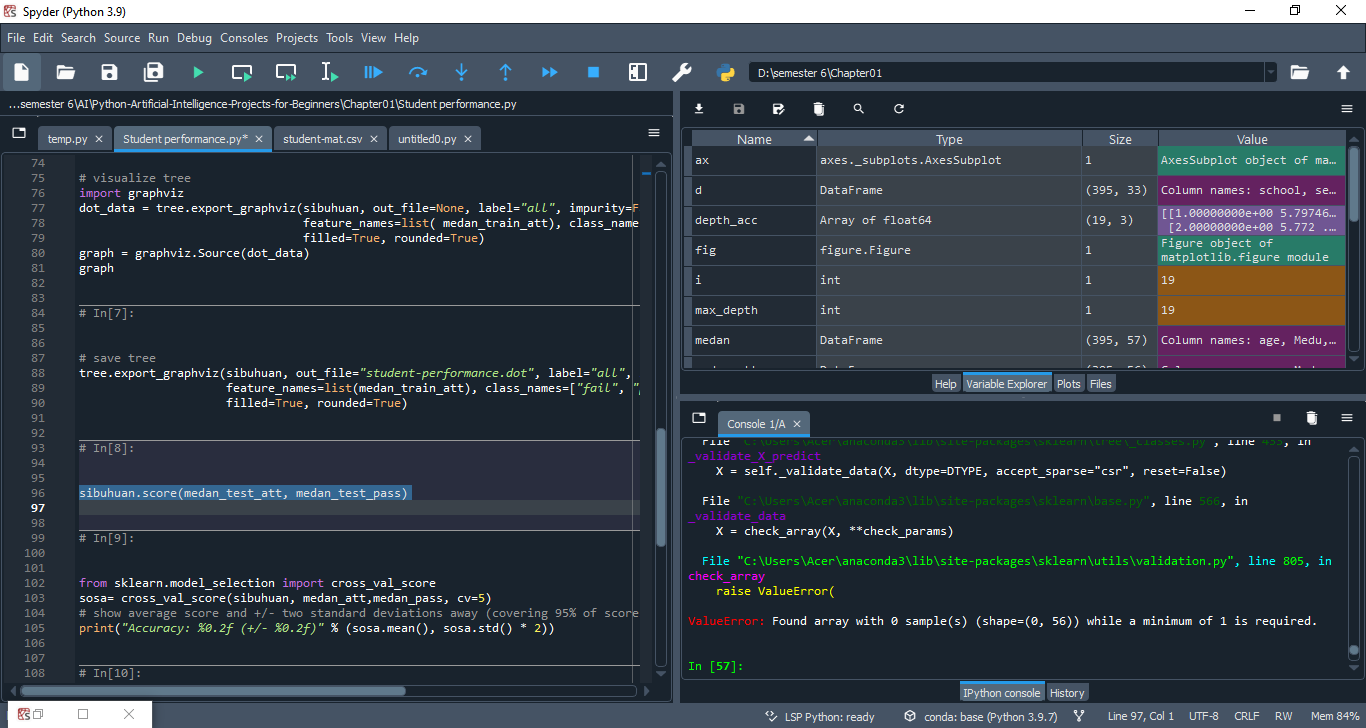
\includegraphics[scale=0.4]{figures/chapter 2/8.PNG}
\end{figure}
\newpage
\item
\begin{verbatim}
	from sklearn.model_selection import cross_val_score
	scores = cross_val_score(t, d_att, d_pass, cv=5)
	# show average score and +/- two standard deviations away 
	#(covering 95% of scores)
	print("Accuracy: %0.2f (+/- %0.2f)" % (scores.mean(), scores.std() * 2))
\end{verbatim}
\begin{figure}[!htbp]
	\centering
	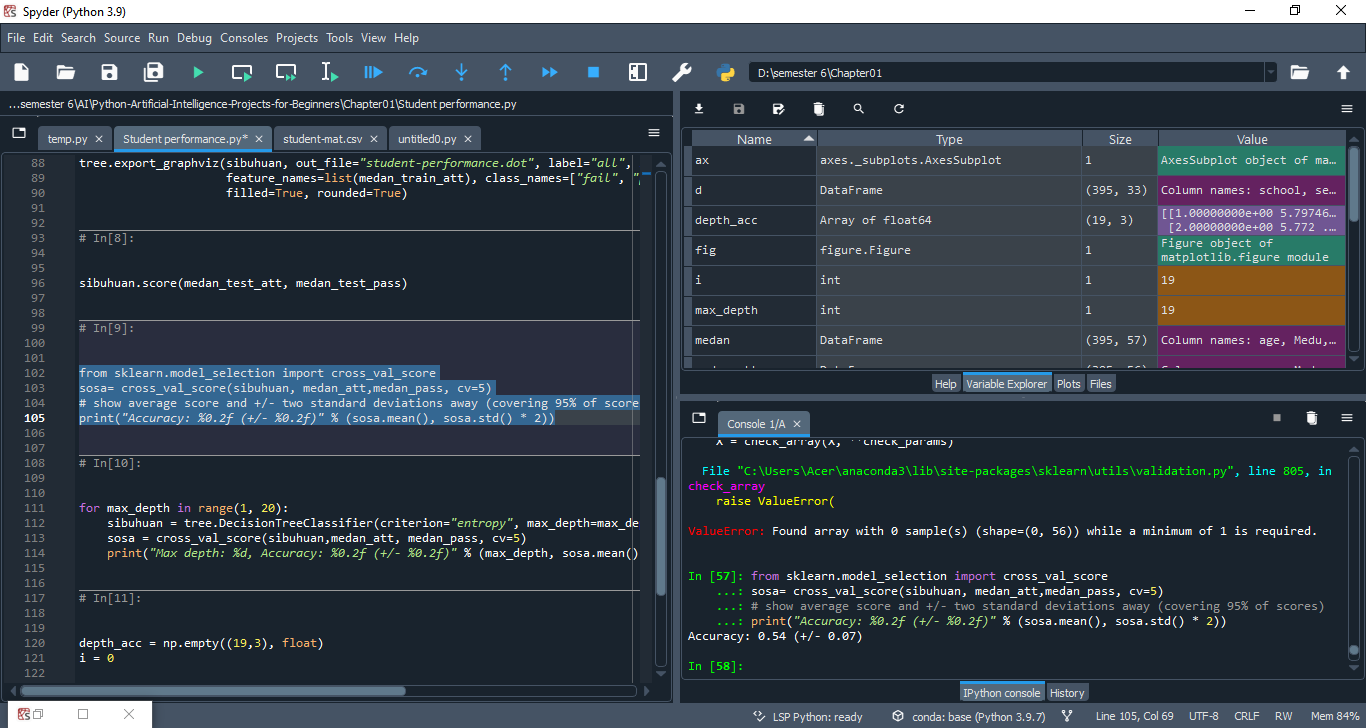
\includegraphics[scale=0.4]{figures/chapter 2/9.PNG}
\end{figure}
\newpage
\item 
\begin{verbatim}
	for max_depth in range(1, 20):
	    t = tree.DecisionTreeClassifier(criterion="entropy", 
			max_depth=max_depth)
	    scores = cross_val_score(t, d_att, d_pass, cv=5)
	    print("Max depth: %d, Accuracy: %0.2f (+/- %0.2f)" % 
				(max_depth, scores.mean(), scores.std() * 2)
			 )
\end{verbatim}
\begin{figure}[!htbp]
	\centering
	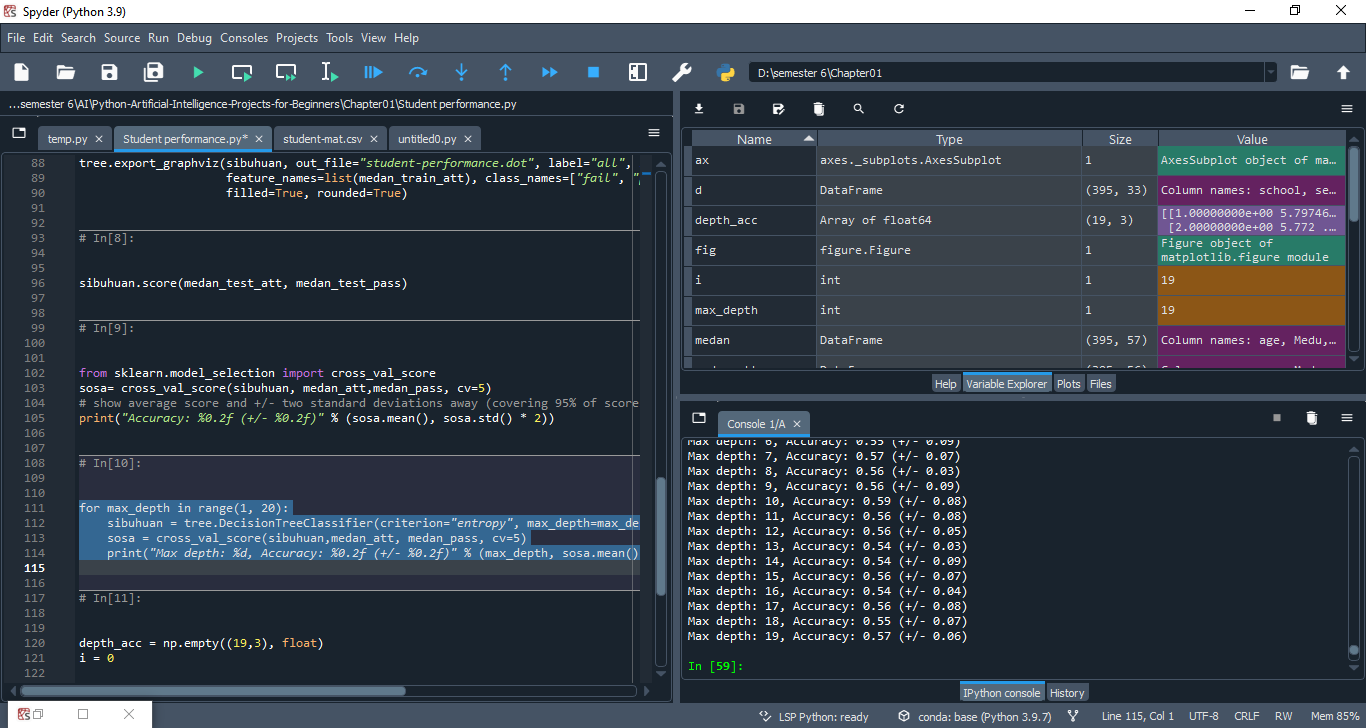
\includegraphics[scale=0.4]{figures/chapter 2/10.PNG}
\end{figure}
\newpage
\item
\begin{verbatim}
	depth_acc = np.empty((19,3), float)
	i = 0
	for max_depth in range(1, 20):
	    t = tree.DecisionTreeClassifier(criterion="entropy", 
			max_depth=max_depth)
	    scores = cross_val_score(t, d_att, d_pass, cv=5)
	    depth_acc[i,0] = max_depth
	    depth_acc[i,1] = scores.mean()
	    depth_acc[i,2] = scores.std() * 2
	    i += 1

	depth_acc
	\begin{figure}[!htbp]
		\centering
		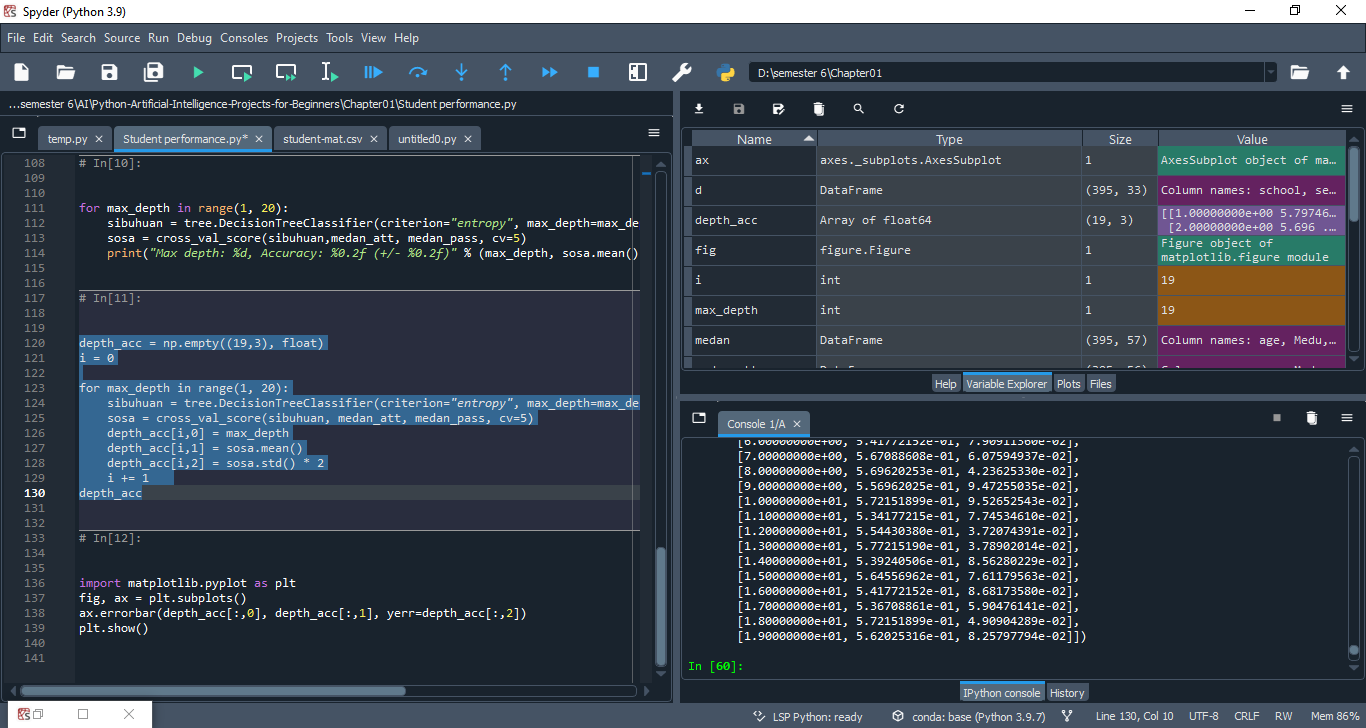
\includegraphics[scale=0.4]{figures/chapter 2/11.PNG}
	\end{figure}
	\newpage
\end{verbatim}
\item 
\begin{verbatim}
	import matplotlib.pyplot as plt
	fig, ax = plt.subplots()
	ax.errorbar(depth_acc[:,0], depth_acc[:,1], yerr=depth_acc[:,2])
	plt.show()
\end{verbatim}
\begin{figure}[!htbp]
	\centering
	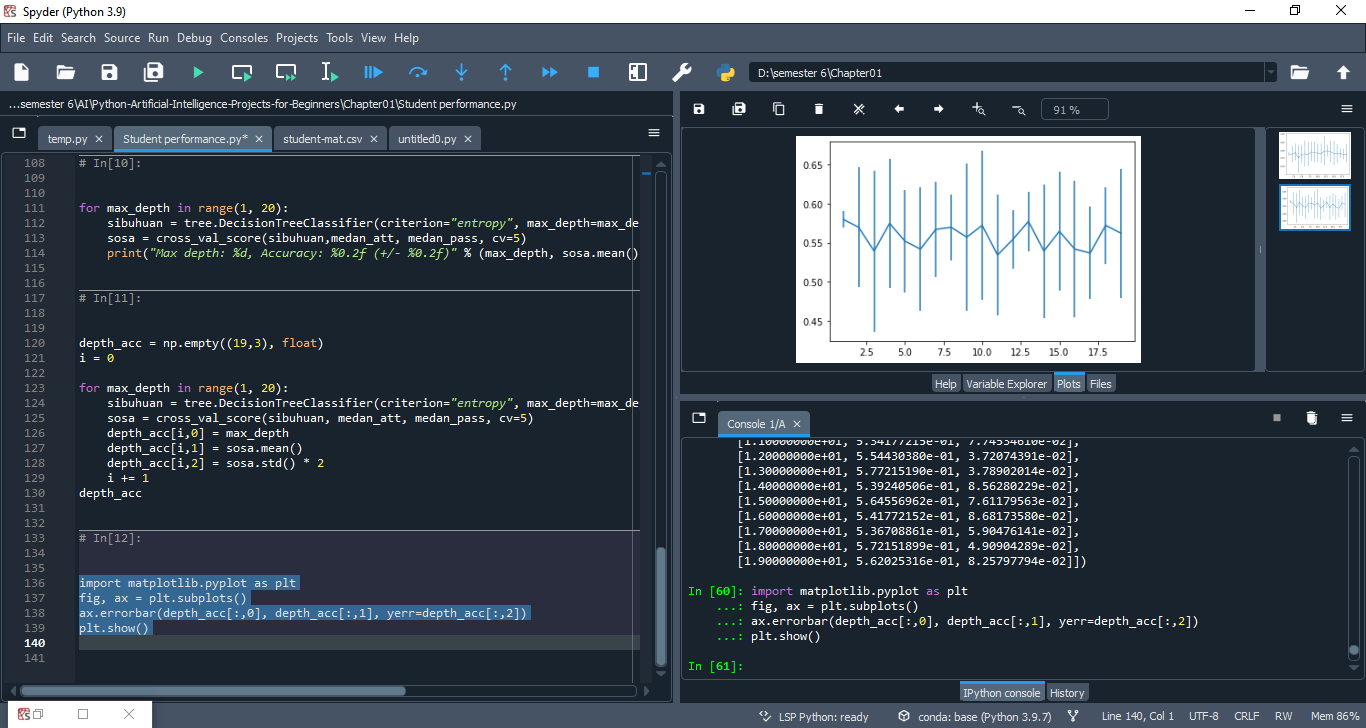
\includegraphics[scale=0.4]{figures/chapter 2/12.PNG}
\end{figure}
\newpage

\end{enumerate}


\section{Penanganan Error}
Dari percobaan yang dilakukan di atas, error yang kita dapatkan di dokumentasikan dan di selesaikan(nilai 5 hari kedua):

\begin{enumerate}
	\item
skrinsut error
	\item
Tuliskan kode eror dan jenis errornya
	\item
Solusi pemecahan masalah error tersebut

\end{enumerate}

